\chapter{Estado del Arte}
La evolución de los sistemas de semaforización inteligente en los últimos años ha sido de forma exponencial, lo que trae nuevas tecnologías, nuevos paradigmas, nuevos prototipos y nuevos esquemas, en este documento se analizará los protocolos de comunicación enfocados a la movilidad vehicular, para luego centrarce en solo los protocolos NTCIP, SCATS, y OCIT; al igual se enfoca a tecnologías de energías renovables, puesto que el modulo planteado trabaja bajo esquemas de energía solar, otra de las tecnologías trabajadas es la tecnología ZIGBEE.

\section{El sistema SCOOT}
(Técnica de Optimización de los valores de Desplazamiento, Ciclo y Giro) se fundamenta en la experiencia aportada por la Red de Tráfico TRANSYT. Lo positivo de este sistema es que realiza una optimización a tres niveles: giro, ciclo y desplazamiento. Utiliza los datos de los detectores de desplazamiento, normalmente detectores de lazo enterrados en el pavimento. Mide el tráfico en tiempo real y desarrolla un modelo de flujo de demanda a cada intersección. Esta secuencia se contrasta con el flujo de salida y de vehículos encolados. Los ajustes temporales son pequeños y no se adaptan a los picos de tráfico, salvo que sea un aumento continuo. Este modelo es utilizado en grandes urbes como Toronto, Madrid, Reino Unido, y para el caso colombiano en Cartagena\cite{15}.

\section{El sistema SCATS}
Se compone de tres niveles, un computador central para realizar la monitorización del sistema global, computadores regionales remotos o locales y controladores locales de señales de tráfico. Su objetivo es la reducción de paradas y retraso, mejorando los tiempos de las rutas. 
El computador central permite el acceso a los computadores regionales para la  recogida de datos de tráfico, datos de entrada y acciones de monitorización.\cite{15}.
\begin{figure}[h]
    \centering
    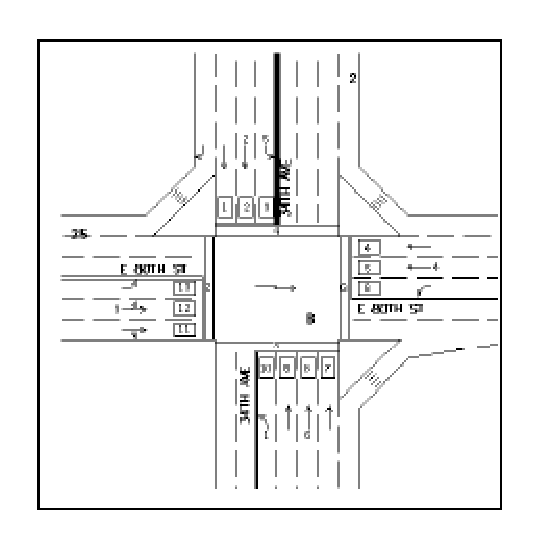
\includegraphics[width=0.4\textwidth]{ima/cruce_phpcUjY57}
    \caption{Sensores para sistema SCATS \cite{18}}
    \label{fig:mesh7}
\end{figure}

\begin{figure}[h]
    \centering
    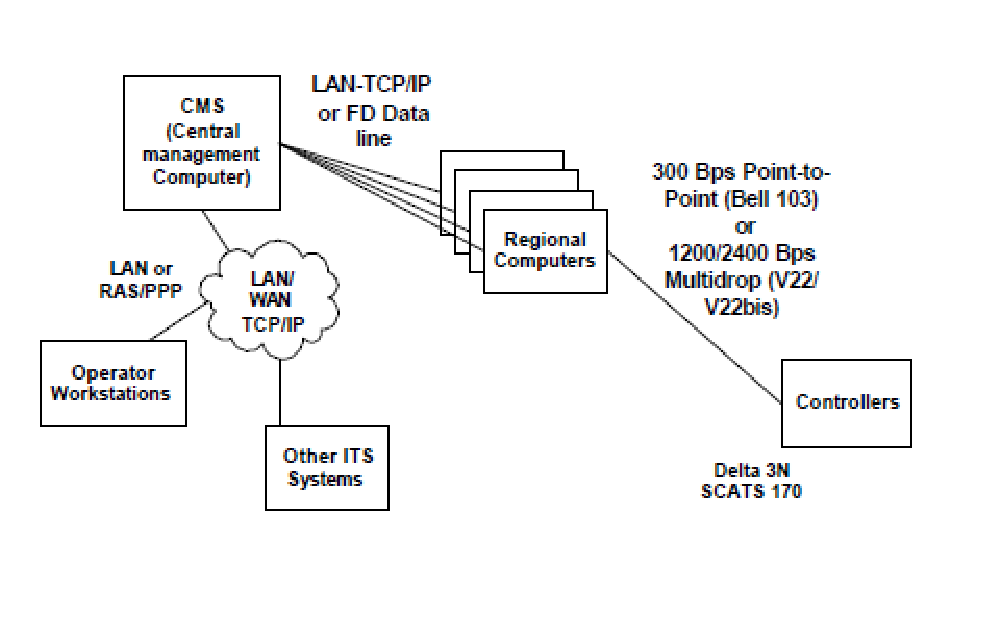
\includegraphics[width=0.8\textwidth]{ima/scat_php1eUteh}
    \caption{Esquema Básico del protocolo SCATS \cite{18}}
    \label{fig:mesh8}
\end{figure}
\section{Sistema NTCIP} 
Dicho sistema cuenta con varias versiones sobre el mismo desarrollo, fue implementado por compañías estadounidenses, dentro del mismo país, este sistema cuenta con varias características:
\subsection{Interoperabilidad}
La interoperatividad refleja la capacidad de múltiples sistemas y dispositivos de diferentes tipos de centros de intercambio información para un propósito común. La interoperabilidad permite que los componentes del sistema de diferentes  proveedores para comunicarse entre sí para proporcionar las funciones del sistema y para trabajar juntos como un sistema completo. Por ejemplo, utilizando la infraestructura mismas comunicaciones para interconectar un sistema de gestión con el tráfico controladores de señal, señales de mensajes dinámicos, controles de vigilancia de vídeo y otros dispositivos para gestionar el tráfico refleja un ejemplo real mundo de interoperabilidad.
\subsection{Intercambiabilidad}
La intercambiabilidad refleja la capacidad de intercambiar dispositivos del mismo tipo en la misma canal de comunicaciones y que dichos dispositivos interactuar con otros dispositivos del mismo tipo que utiliza funciones basadas en estándares. Con capacidad de intercambio, los componentes del sistema pueden modificarse a cabo (conmutada) con componentes similares de diferentes fabricantes, ya que poseen común funcional y física características. Un ejemplo de intercambiabilidad es un controlador de señales de diferentes fabricantes que interactúan entre sí para  proporcionar la coordinación de señales de tráfico a lo largo de un camino pasante arterial[16]. 
\subsection{Centro de Campo (C2F) Comunicaciones}
NTCIP proporciona estándares de comunicaciones de dos tipos diferentes para sus comunicaciones. El primer tipo es entre un sistema central y  múltiples dispositivos de control o de vigilancia gestionado por la central. Un ejemplo de un sistema central es un ordenador en el seguimiento  y el control de la operación de controladores basados en microprocesadores de carretera para las señales de tráfico dentro de una ciudad. El sistema central puede enviar instrucciones a los controladores de semáforos para cambiar configuraciones de cronometraje, las condiciones de circulación y el envio de información de  los estados del tráfico a la computadora. Otros ejemplos de este tipo de comunicaciones incluyen.
\begin{itemize}
    \item Un sistema de transporte a bordo del vehículo se comunica con un dispositivo de señales de tráfico para facilitar la prioridad de tránsito.
    \item  Un sistema de gestión de la autopista que comunica con los detectores y medidores de rampa en las autopistas.
    \item El control de sistema de gestión de tráfico de un camino de iluminación, circuito cerrado de televisión (CCTV), las señales de mensajes dinámicos, transmisores de radio de asesoramiento, sensores ambientales y estaciones de volumen de tráfico en las carreteras. 
\end{itemize}
Como la mayoría de aplicaciones de este tipo implican un sistema de centro de la comunicación con varios dispositivos en la carretera o en los  vehículos de la agencia, este tipo de comunicación se denomina "centro de campo" (C2F). Los protocolos NTCIP destinados a esta aplicación se utiliza a menudo en un entorno donde un sistema de centro, rutinariamente encuesta cada dispositivo de campo, como en el caso más común de múltiples dispositivos de campo, se suele compartir un canal de comunicaciones.
\subsection{Centro de Centro de Comunicaciones (C2C)}
El segundo tipo de comunicación implica los mensajes enviados entre dos o más sistemas de centro. Este tipo de comunicación se denomina centro a centro de comunicaciones (C2C), aunque dos o más de los diversos sistemas pueden de hecho, estar situados dentro de la misma "central" o edificio, son lógicamente separados. C2C implica comunicaciones de igual a igual entre cualquier número de sistemas de centros en un muchos a muchos de una red. Este tipo de comunicación es similar a la Internet, en que cualquier centro puede solicitar información de, o proporcionar información a, cualquier número de otros centros. Un ejemplo de las comunicaciones C2C es de dos centros de gestión de tráfico que intercambian en tiempo real información sobre el inventario y el estado de los dispositivos de control de tráfico. Esto permite que cada sistema de centro sabe qué plan de tiempo, por ejemplo, el otro sistema central está en marcha para permitir la coordinación de señales de tráfico allá de las fronteras geográficas del centro \cite{16}.

\begin{figure}[H]
    \centering
    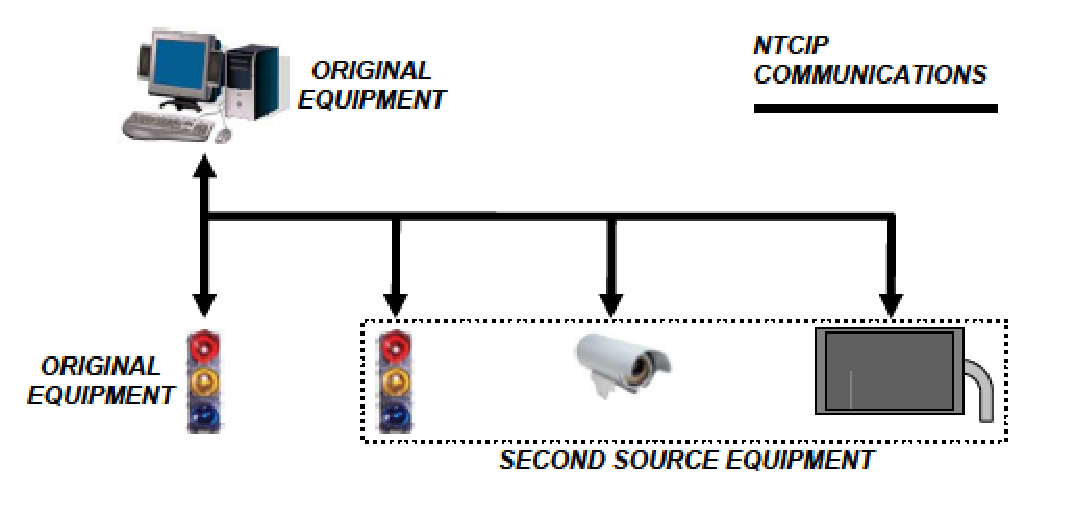
\includegraphics[width=1\textwidth]{ima/ntc_php4gbMlF}
    \caption{Propiedades e imteroperatividad e intercambiabilidad de NTCIP\cite{9}}
    \label{fig:mesh9}
\end{figure}
\begin{figure}[H]
    \centering
    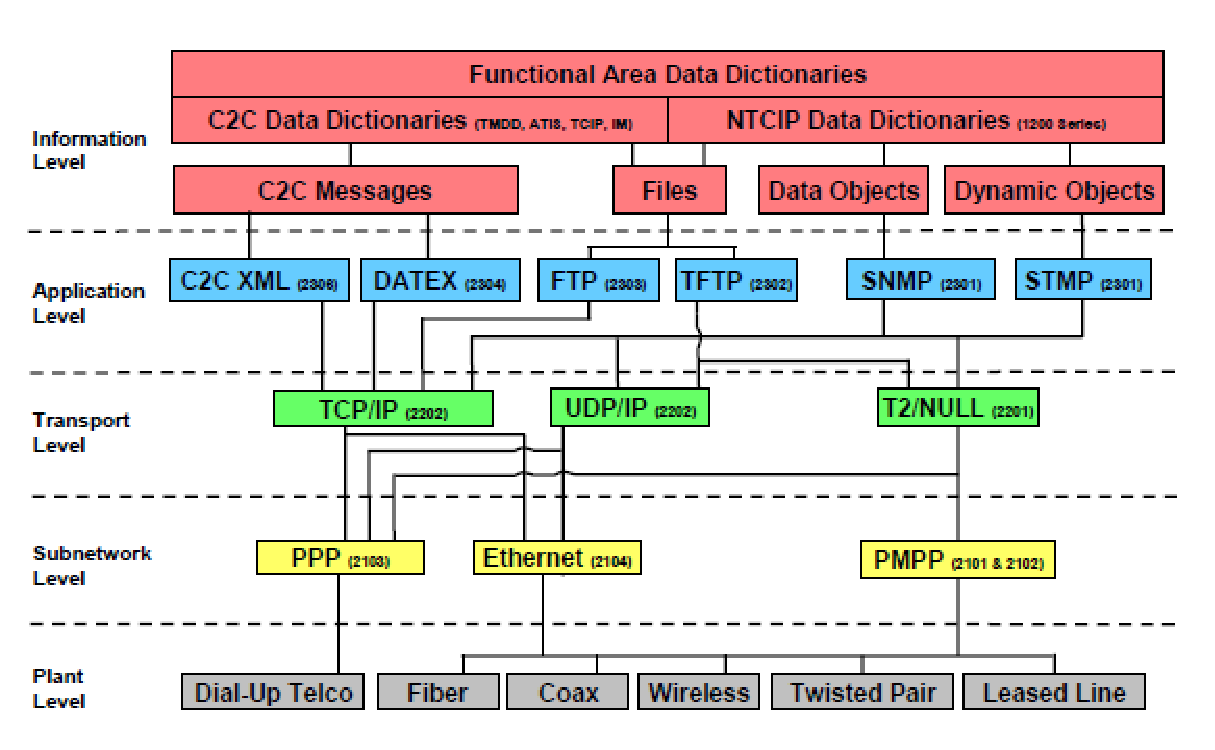
\includegraphics[width=0.8\textwidth]{ima/ntc1_phpfqEM84}
    \caption{NTCIP Framework \cite{9}}
    \label{fig:mesh10}
\end{figure}
\begin{figure}[H]
    \centering
    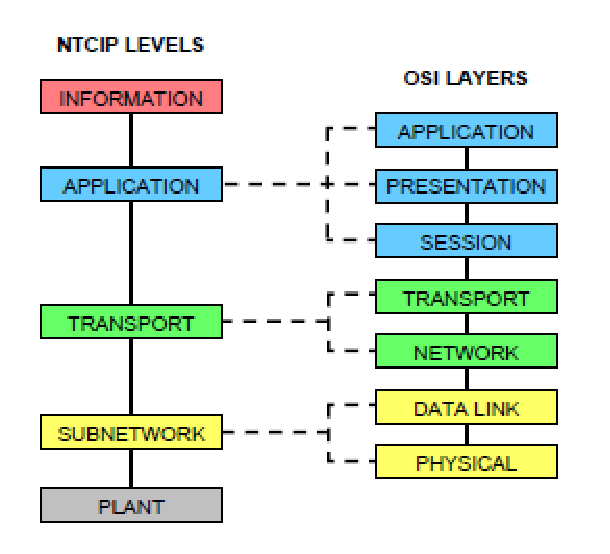
\includegraphics[width=0.6\textwidth]{ima/ntc2_phpj0fRQP}
    \caption{Mapa capas OSI a capas NTCIP \cite{9}}
    \label{fig:mesh11}
\end{figure}
\newpage
\newpage


\section{Sistema OCIT}
Para el sistema OCIT el cual fue incorporado en algunas ciudades de Alemania, se tienen las siguientes características:
\begin{itemize}
    \item Protocolo de conversión basado en el estándar SOAP con un simple patrón de petición-respuesta en la comunicación (recuperación directa de los datos).
    \item Definición de un modelo de datos global en la región de datos de proceso que abarca todas las ramas del sistema de enrutamiento de control de tráfico y el tráfico, el uso de la OCIT-I modelo de datos para los SAT. La funcionalidad del modelo de datos de la OCIT-I es retratado en su totalidad.
    \item Integración de sistemas y los ajustes deseados se regulan previamente como parte de la planificación del proyecto.
    \item Pruebas de conformidad del protocolo se llevan a cabo en un entorno de prueba que se proporciona el uso de OCIT. Las pruebas de todas las implementaciones de protocolo (contenido y datos) se llevan a cabo sobre una base de proyecto por proyecto.
    \item Las actualizaciones incluyen componentes de DATEX II pueden ser posibles dependiendo de retomar proyecto de requisitos.
    \item Las actualizaciones incluyen componentes de DATEX II pueden ser posibles dependiendo de retomar proyecto de requisitos.
    
\end{itemize}

 La interfaz de comunicación debe aplicarse de la misma manera en todas las unidades centrales. Para ello, el protocolo SOAP se utiliza como una interfaz de comunicación de nivel superior, a través de la cual toda la comunicación se lleva a cabo. La forma descrita aquí se designa como un protocolo OCIT-C.
 Esta interfaz OCIT-C está abierta y se puede utilizar en diversos sistemas, en su mayor parte en el área de los sistemas de control de tráfico. Es el propósito de este documento para describir el protocolo OCIT-C y su uso. No se va a describir los datos estructurales de los datos a transmitir. Esto se describe en el documento "OCIT-C de datos".
 Este sistema se incorpora bajo el siguiente esquema de conexión y de interactividad \cite{17}.
 \begin{figure}[h]
    \centering
    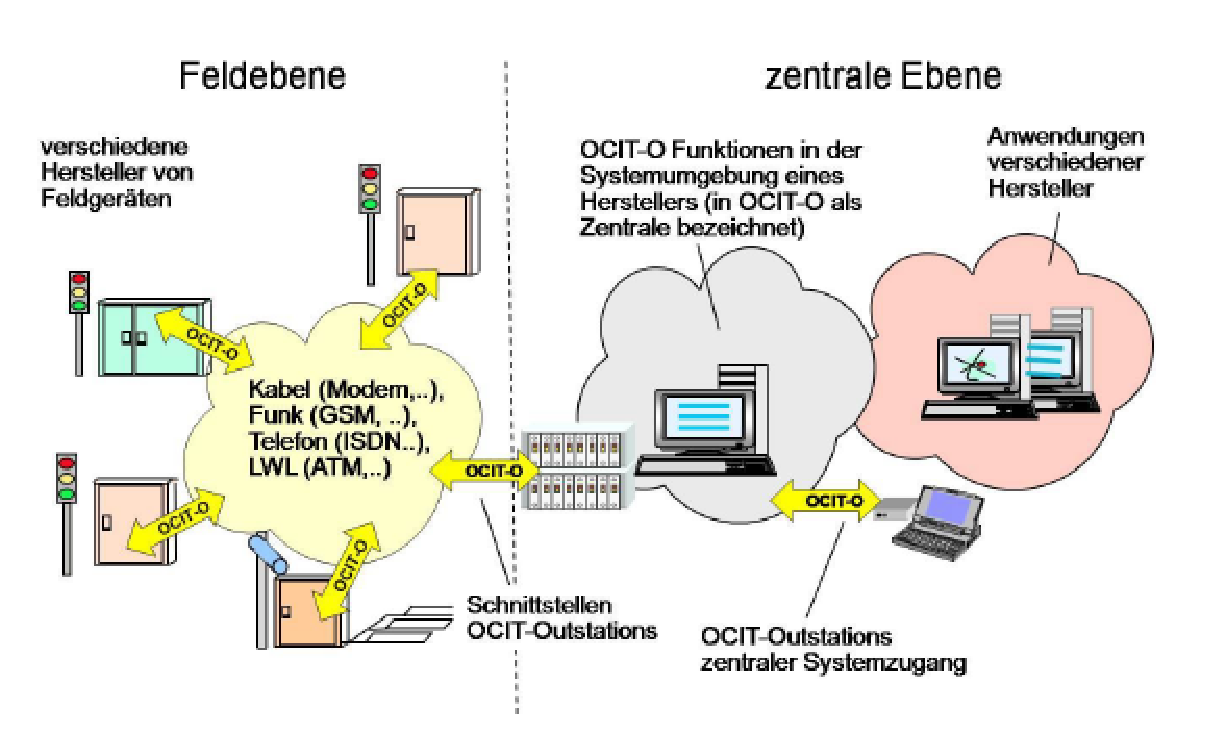
\includegraphics[width=1\textwidth]{ima/ocit_php7K8DbI}
    \caption{Esquema general de OCIT-C \cite{11}}
    \label{fig:mesh12}
\end{figure}
 El siguiente gráfico muestra como se comunica los servidores con los clientes, siendo una interactividad de tipo bidireccional.
 \begin{figure}[h]
    \centering
    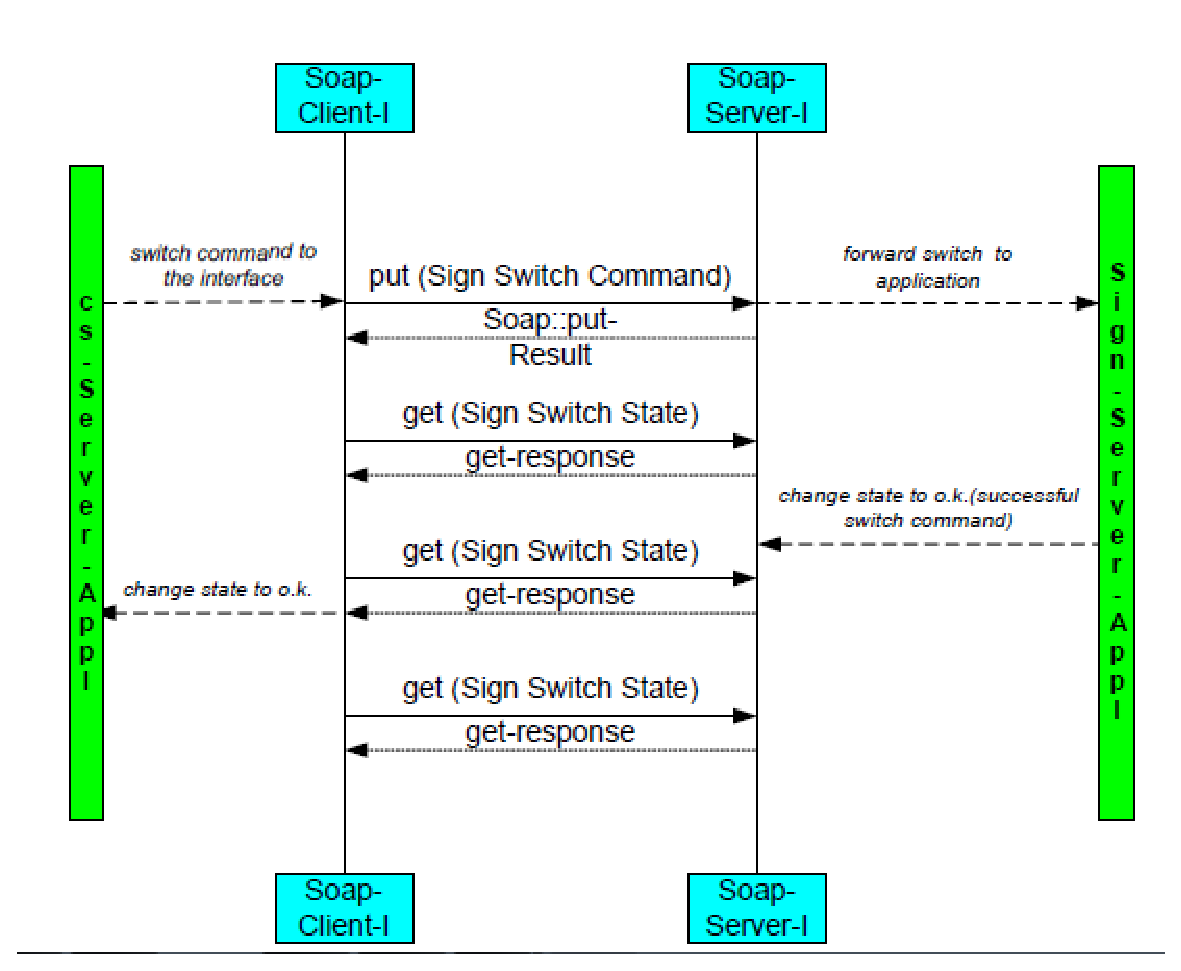
\includegraphics[width=0.8\textwidth]{ima/ocit1_phpVmReMk}
    \caption{Estado regular de la comunicación \cite{17}}
    \label{fig:mesh13}
\end{figure}
 En resumidas cuentas y palabras el protocolo se describe como 4 capas, al estilo del protocolo OSI\cite{17}.

\begin{figure}[h]
    \centering
    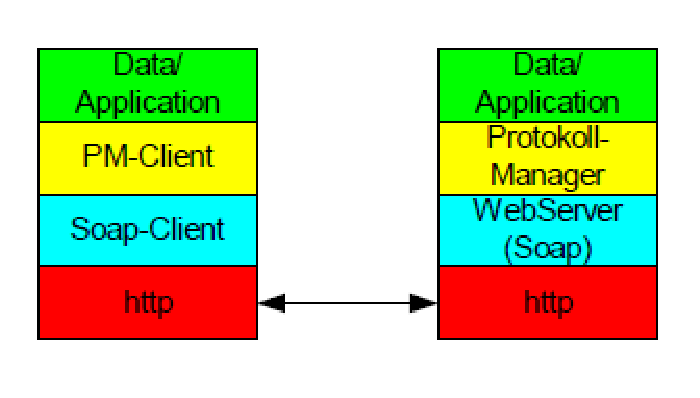
\includegraphics[width=0.6\textwidth]{ima/ocit2_phplDTo60}
    \caption{Capas cliente- servidor OCIT-C \cite{17}}
    \label{fig:mesh14}
\end{figure}
\newpage
\section{Tecnología ZBEE}
ZigBee, también conocido como "HomeRF Lite", es una tecnología inalámbrica con velocidades comprendidas entre 20 kB/s y 250 kB/s.· Los rangos de alcance son de 10 m a 75 m\cite{12}.
\begin{itemize}
    \item Puede usar las bandas libres ISM (6) de 2,4 GHz (Mundial), 868 MHz (Europa) y 915 MHz (EEUU).
    \item  Una red ZigBee puede estar formada por 255 nodos los cuales tienen la mayor parte del tiempo el transceiver ZigBee dormido con objeto de consumir menos energía que otras tecnologías inalámbricas.
    \item Un sensor equipado con un transceiver ZigBee pueda ser alimentado con dos pilas AA durante al menos 6 meses y hasta 2 años.
    \item La fabricación de un transmisor ZigBee consta de menos circuitos analógicos de los que se necesitan habitualmente.
    \item  Diferentes tipos de topologías como estrella, punto a punto, malla, árbol.
    \item Acceso de canal mediante CSMA/CA(7) (acceso múltiple por detección de portadora con evasión de colisiones).
    \item Escalabilidad de red -- Un mejor soporte para las redes más grandes, ofreciendo más opciones de gestión, flexibilidad y desempeño.
    \item  Fragmentación -- Nueva capacidad para dividir mensajes más largos y permitir la interacción con otros protocolos y sistemas.
    \item  Agilidad de frecuencia -- Redes cambian los canales en forma dinámica en caso que ocurran interferencias.
    \item Gestión automatizada de direcciones de dispositivos.
    \item  El conjunto fue optimizado para grandes redes con gestión de red agregada y herramientas de configuración.
    \item Localización grupal -- Ofrece una optimización adicional de tráfico necesaria para las grandes redes.
    \item  Instalación de servicio inalámbrico -- El modulo fue mejorado con capacidades para poner en marcha el servicio inalámbrico.
    \item Recolección centralizada de datos -- El modulo fue sintonizado específicamente para optimizar el flujo de información en las grandes redes.    
\end{itemize}
    
\subsubsection{Ventajas}
\begin{itemize}
\item Ideal para conexiones punto a punto y punto a multipunto.
\item Diseñado para el direccionamiento de información y la actualización de la red.
\item  Opera en la banda libre de ISM 2.4 Ghz para conexiones inalámbricas.
\item  Óptimo para redes de baja tasa de transferencia de datos.
\item  Alojamiento de 16 bits a 64 bits de dirección extendida.
\item  Reduce tiempos de espera en el envío y recepción de paquetes.
\item  Detección de Energía (ED).
\item  Ciclo de trabajo mínimo - Proporciona larga duración de la batería.
\item  Soporte para múltiples topologías de red: Estática, dinámica, estrella y malla.
\item Hasta 65.000 nodos en una red.
\item  Cifrado AES de 128-bit - Provee conexiones seguras entre dispositivos.
\item Son más baratos y de construcción más sencilla.
\end{itemize}
\subsubsection{Desventajas}
\begin{itemize}
\item La tasa de transferencia es muy baja.
\item Solo manipula textos pequeños comparados con otras tecnologías.
\item Zigbee trabaja de manera que no puede ser compatible con bluetooth en todos sus aspectos porque no llegan a tener las mismas tasas de transferencia, ni la misma capacidad de soporte para nodos.
\item  Tiene menor cobertura porque pertenece a redes inalámbricas de tipo WPAN\cite{12}.
\end{itemize}
\begin{figure}[h]
    \centering
    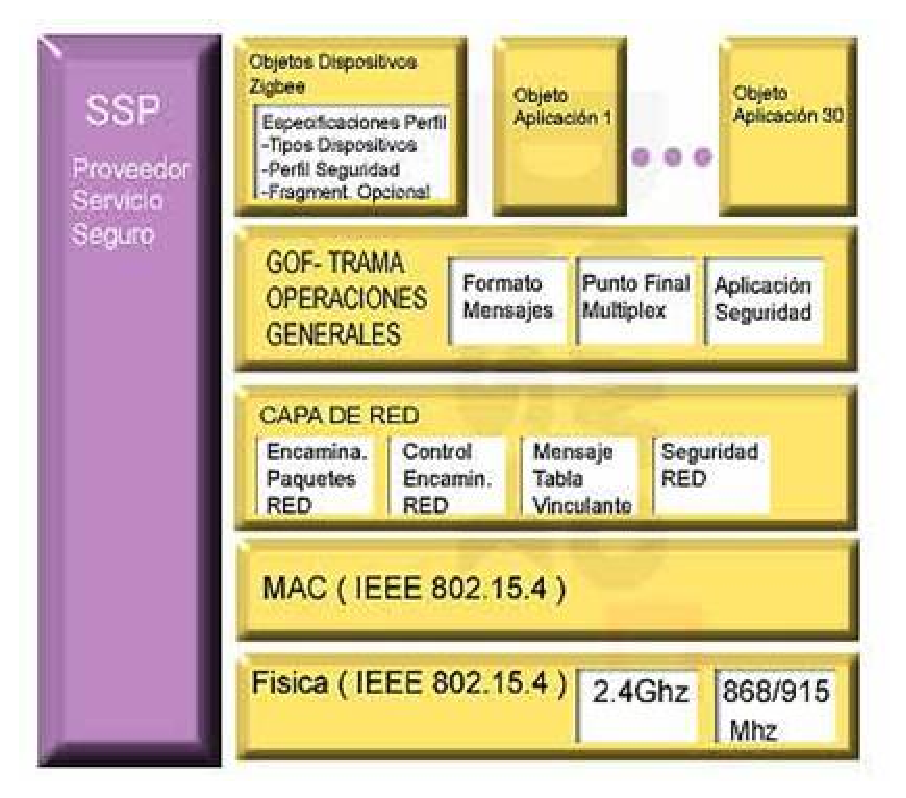
\includegraphics[width=1\textwidth]{ima/z1_phpBkhYj6}
    \caption{Estructura ZIGBEE \cite{12}}
    \label{fig:mesh15}
\end{figure}